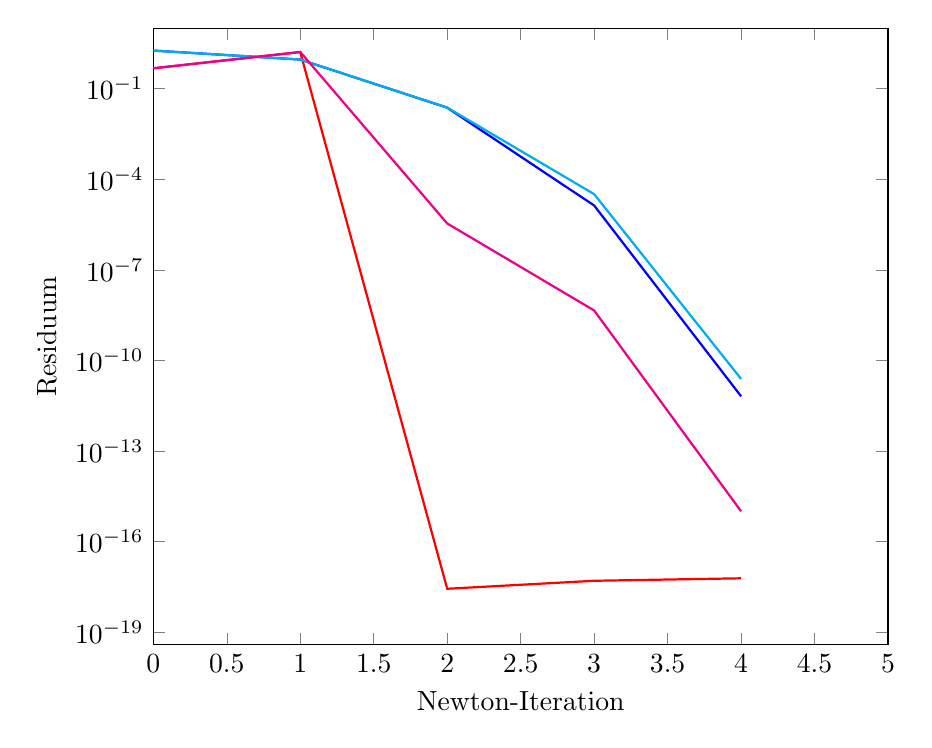
\begin{tikzpicture}[every plot/.append style={thick}] 
\begin{axis}[ 
label style={font=\normalsize}, 
xlabel={Newton-Iteration}, 
ylabel={Residuum}, 
xmin=0, xmax=5, 
ymode=log, 
ymin=0, ymax=10, 
width=0.9\textwidth, 
grid style=dashed, 
] 
\addplot[ 
color=blue, 
] 
coordinates { 
(0, 1.82e+00)(1, 9.17e-01)(2, 2.34e-02)(3, 1.35e-05)(4, 6.49e-12)}; 
\addplot[ 
color=red, 
] 
coordinates { 
(0, 4.71e-01)(1, 1.62e+00)(2, 2.75e-18)(3, 5.06e-18)(4, 6.11e-18)}; 
\addplot[ 
color=cyan, 
] 
coordinates { 
(0, 1.82e+00)(1, 9.17e-01)(2, 2.36e-02)(3, 3.21e-05)(4, 2.44e-11)}; 
\addplot[ 
color=magenta, 
] 
coordinates { 
(0, 4.72e-01)(1, 1.64e+00)(2, 3.43e-06)(3, 4.51e-09)(4, 1.01e-15)}; 
\end{axis} 
\end{tikzpicture} 
